\chapter{Аналитический раздел}

В данном разделе будут выдвинуты требования к приложению, определены пользователи системы, формализованы хранимые о системе данные, а также проведен анализ существующих решений.

\section{Требования к приложению}

Приложение должно поддерживать определенный функционал:
\begin{itemize}
	\item персонализация пользователей;
	\item создание новых заявок и изменение информации об уже существующих;
	\item добавление оборудования;
	\item добавление навыков и отправка их на подтверждение;
	\item пополнение списка ролей конкретного пользователя и переключение между ними.
\end{itemize}

\section{Пользователи системы}

Для работы с системой обязательным этапом является прохождение персонализации. Пользователь может работать в системе под одной из следующих ролей.
\begin{enumerate}
	\item Оформитель -- пользователь, обладающий возможностями создания заявки, изменения ее параметров, закрытия заявки.
	\item Исполнитель -- пользователь, обладающий возможностями отправления своих навыков на подтверждение, взятия заявок на исполнение и их последующего закрытия.
	\item Администратор -- пользователь, обладающий возможностью подтверждения роли других администраторов и профессиональных навыков исполнителей.
\end{enumerate}
В ходе использования приложения предусмотрена возможность смены ролей.
На рисунке \ref{use-case} представлена диаграмма использования приложения.

\begin{figure}[H]
	\begin{center}
		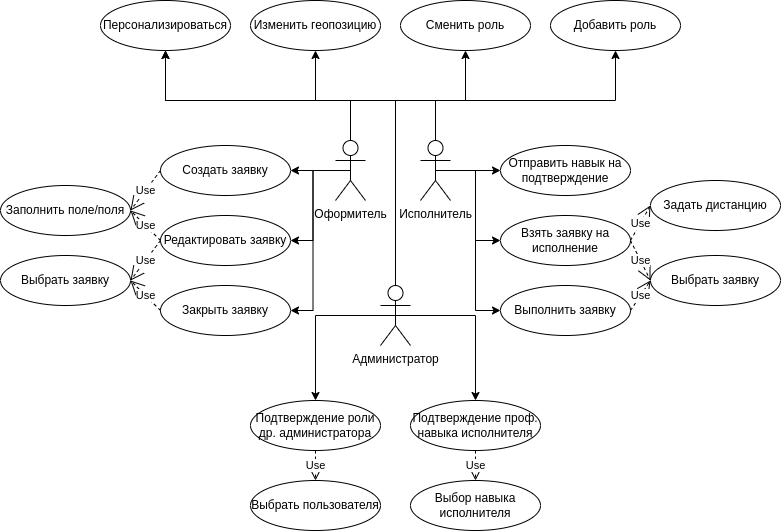
\includegraphics[scale=0.6]{assets/use-case.png}
	\end{center}
	\caption{Use-case диаграмма}
	\label{use-case}
\end{figure}

\section{Формализация данных}

База данных состоит из нескольких таблиц:
\begin{itemize}
	\item таблица пользователей User;
	\item таблица подключений Connection;
	\item таблица заявок Request;
	\item таблица оборудования Equipment;
	\item таблица навыков Skill;
	\item таблица, реализующая связь <<многие ко многим>> для исполнителей и навыков ExecutorSkill;
	%\item таблица, реализующая связь <<многие ко многим>> для оборудования и навыка EquipmentSkill;
	\item таблица, хранящая набор данных для предотвращения использования ненормативной лексики Ban.
\end{itemize}
На рисунке \ref{er-chen} представлена ER-диаграмма сущностей в нотации Чена.

\begin{figure}[H]
	\begin{center}
		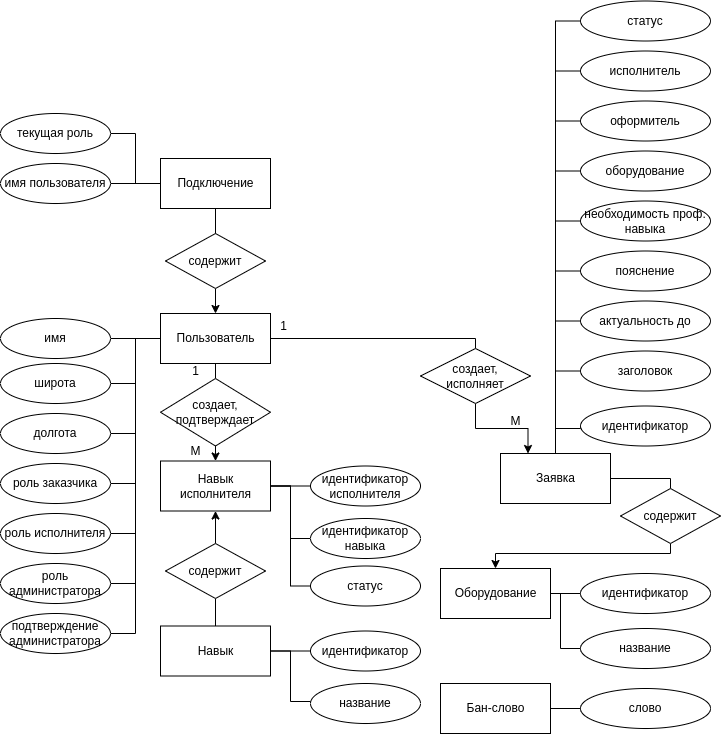
\includegraphics[scale=0.6]{assets/ER-Chen.png}
	\end{center}
	\caption{ER-диаграмма в нотации Чена}
	\label{er-chen}
\end{figure}

\section{Анализ существующих решений}

Среди уже имеющихся проектов, решающих поставленную задачу, были выделены 3 аналога (таблица \ref{decisions}). Сравнение проводилось по ряду критериев, а именно авторизация, наличие территориальной привязки, охват аудитории, а также были выделены преимущественные особенности системы.

\begin{table}[H]
	\centering
	\caption{Существующие решения поставленной задачи}
	\label{decisions}
	\begin{tabular}{|p{2.3cm}|p{3.3cm}|p{3cm}|p{3cm}|p{3.1cm}|}
		\hline
		\textbf{Название проекта} & \textbf{Авторизация} & \textbf{Наличие территориальной привязки} & \textbf{Охват аудитории} & \textbf{Особенности системы}\\
		\hline 
		\textbf{YouDo \cite{youdo}} & Электронная почта или Вконтакте, Одноклассники, Google, Mail, Apple & На уровне города & Более 2.5 миллионов пользователей & Заказо- ориентирован- ность со стабильной системой отзывов\\
		\hline
		\textbf{Все соседи \cite{all_neighbour}} & Номер телефона & Устанавлива- ется с точностью до дома & Около 60 тыс. пользователей & Бартерная система взаимовыручки\\
		\hline
		\textbf{Привет, сосед! \cite{hello_neighbour}} & Электронная почти или Вконтакте, Facebook, Одноклассники, Google, Yandex, Apple & Устанавлива- ется с точностью до дома & Около 2 тыс. пользователей & Уклон в социальную сеть с бонусной программой \\
		\hline
	\end{tabular}
\end{table}

Стоит упомянуть, что все вышеуказанные решения имеют мобильные версии для IOS и Android, а также Web-версии приложений.

У каждого вышеупомянутого аналога имеются недостатки среди выделенных критериев, как например слабоконкретизированная геопозиция, неудобная авторизация или малое количество участников. Избавиться от первого из них не составляет труда (стоит повысить точность геолокации), тогда как последние два могут быть сведены к использованию популярного мессенджера, имеющего большой охват аудитории. Таким вариантом можно смело назвать telegram, который не уступает приведенным проектам в кроссплатформенности.

\section{Вывод из раздела}

В данном разделе были выделены ролевые модели системы, конкретизированы хранимые данные и их связь между собой, построены соответствующие диаграммы. Также был проведен анализ существующих на рынке решений, который позволил понять, каких особенностей в них не хватает.